\section{Methods and Experimental Setup Details}
\label{app:experimental_setup}

\subsection{ReMIA Details}
\label{app:remia_details}
ReMIA trains a tabular discriminator to distinguish between synthetic data from two different sources, and it is then applied to a non-intersecting subset of the training records of each source to assess the information leakage of the synthetic data.
Inputs are preprocessed as follows: numerical features are standardized using training-set mean and standard deviation, and categorical features are one-hot encoded (unknown categories are mapped to zero vectors of the same dimension).
The discriminator is a multilayer perceptron with two hidden layers (100 and 50 units), SiLU activations \citep{elfwing2018sigmoid}, and layer normalization \citep{ba2016layer} applied before each hidden layer. The output layer has a single unit with sigmoid activation.

Optimization uses RAdam \citep{loshchilov2017decoupled} with learning rate $5\times 10^{-3}$ and binary cross-entropy. Training runs for at most $1000$ epochs, with batch size $500$ and early stopping on training loss with patience $50$.
The AUROC score is computed on the training set, and on the target records every 2 steps, using the discriminator's predicted probabilities as membership scores. In order to improve stability and reduce noise, AUROC scores are smoothed by a centered rolling mean with a window equal to $10\%$ of the recorded steps.


\subsection{Baseline Privacy Metrics}
\label{app:baseline_privacy_metrics}

\paragraph{DCR.}
Given a distance function $d$, a record $x$ and a dataset $\data$, we define the distance to closest record (DCR) as $\text{DCR}(x, \data) = \min_{x' \in \data} d(x, x')$.
In this article, we implement the DCR-based privacy metric following \citet{zhang2024mixed}:
Given training data $\data_t$, synthetic data $\data_s$, hold-out data $\data_h$, and a distance function $d$, we compute for each record $x_i$ in $\data_t$ the DCRs to the synthetic data $\text{DCR}(x_i, \data_s)$ and to the hold-out data $\text{DCR}(x_i, \data_h)$, and we compute the fraction of records in $\data_t$ for which the DCR to the synthetic data is smaller than the DCR to the hold-out data:
\begin{equation}
\frac{1}{|\data_t|} \sum_{x_i \in \data_t} \mathds{1}[\text{DCR}(x_i, \data_s) < \text{DCR}(x_i, \data_h)]
\end{equation}
If this fraction is significantly higher than 50\%, then the synthetic data is considered to be leaking information about the training data.
In our implementation, we use the cosine distance (1 minus the cosine similarity) as the distance function, after standardizing numerical features and one-hot encoding categorical features.


\paragraph{smMIA.}
We use the implementation of the MIA based on shadow modeling as described in \citet{meeus2023achilles}.
In particular, we use the query-based feature extraction \citep{houssiau2022tapas} and a random forest as the predictive model because it represents the most effective attack.
We keep the default settings where the number of training shadow datasets is set to 1000, and the number of test shadow datasets is set to 200. In half of both training and test shadow datasets, the target record is included in the training set of the shadow model, while in the other half it is not. The shadow models are trained for 100 epochs with early stopping on validation loss with patience 10, and the best model is selected based on validation performance.
Data for building the shadow datasets is sampled with replacement from the original dataset, in particular we use two different splits of the original dataset for building the training and test shadow datasets, where the split for the training data is double the size of the split for the test data. In particular, we use all the available data for the Adult and California datasets, while for the UK Census dataset we use a random sample of 75,000 records. Considering training shadow datasets with 1,000 records, this means that the total data usage for running the attack is $\approx20\times$ for California dataset, $\approx40\times$ for Adult dataset, and $\approx75\times$ for the UK Census dataset.

We follow the strategy outlined in \citep{meeus2023achilles} for the selection of the target record, which consists of sorting the records by the average cosine distance for the k-nearest neighbors and selecting the one with the highest distance.
This strategy is based on the intuition that records that are more isolated in the feature space are more vulnerable to MIAs, and thus represent a worst-case scenario for the evaluation of the privacy risk of synthetic data. Indeed, it has been shown that the performance of MIAs is significantly higher on outlier records than on random records \citep{meeus2023achilles}.
In order to evaluate the performance of smMIA on a more typical scenario, we also evaluate the attack on the record with the median distance to its k-nearest neighbors. This makes smMIA more comparable to the other metrics, which are not designed to target single outlier records.
Performing more attacks on different target records would be computationally prohibitive. In many cases, one smMIA takes several hours to be performed. As we later report in Appendix \ref{app:computational_resources}, the total time taken for the experiments shown in this article is approximately 882 hours, of which about 865 hours were spent on attacks based on shadow modeling.

\paragraph{DOMIAS.}
We adapt the original implementation of DOMIAS \citep{van2023membership} to tabular data with discrete features.
To do this, we first encode categorical features with one-hot encoding. Then, we apply principal component analysis (PCA) to avoid linearly dependent features that cause issues when training density estimators.
We use kernel density estimation (KDE) with Gaussian kernel as the density estimator, keeping the settings of the original implementation.
We do not use the block neural autoregressive flow (BNAF) \citep{de2020block} as the density estimator because it is designed for continuous data and from preliminary experiments it performed poorly compared to KDE. This was also observed in the original paper, where the advantage of using BNAF over KDE was emerging only for large training datasets,
making it not competitive considering the substantial increase in computational cost.
Finally, we set the size of the reference (auxiliary) dataset to be 5 times larger than the training set (so in our case 5000 records).
These settings imply a total additional data usage that is 6 times the size of the training set, considering the reference dataset ($5\times$) and the control dataset ($1\times$) containing non-training records used to evaluate the performance.

\subsection{Synthetic Data Generators}
\label{app:sdgs}
We show in Table \ref{tab:sdgs_summary} the list of SDGs used in our experiments, with a reference to their respective publications, the implementation used, and the maximum running time across all experiments (for datasets of size 1,000).
\begin{table}[h]
  \centering
  \caption{Synthetic data generators used in our experiments, with implementation sources and maximum observed runtimes for datasets of size 1,000.}
  \label{tab:sdgs_summary}
  \begin{tabular}{lccc}
    \toprule
    SDG Name & Reference & Implementation & Runtime (seconds)\\
    \midrule
    ADSGAN & \citet{yoon2020anonymization} & synthcity & 222.0 \\
    ARF & \citet{watson2023adversarial} & synthcity & \phantom{0}25.4 \\
    Aindo & - & proprietary & 153.9 \\
    BayNet & \citet{zhang2017privbayes} & rsyn & \phantom{0}14.5 \\
    CTGAN & \citet{xu2019modeling} & rsyn & \phantom{0}16.7 \\
    PateGAN & \citet{jordonpate} & synthcity & 494.2 \\
    PrivBayes($\varepsilon=10$) & \citet{zhang2017privbayes} & rsyn & \phantom{0}14.6 \\
    PrivBayes($\varepsilon=1000$) & \citet{zhang2017privbayes} & rsyn & \phantom{0}16.3 \\
    SynthPop & \citet{nowok2016synthpop} & rsyn & \phantom{00}6.2 \\
    TVAE & \citet{xu2019modeling} & synthcity & \phantom{0}86.0 \\
    TabDDPM & \citet{kotelnikov2023tabddpm} & synthcity & \phantom{0}84.0 \\
    \bottomrule
  \end{tabular}
\end{table}

\subsection{Privacy Risk Models}
\label{app:risk_models}

\paragraph{Leaky model.}
We use the leaky risk model as defined in \citet{palacios2025empirical}: given a training dataset $D_{t}$ and a disjoint dataset of samples from the same distribution $D_{c}$ of the same size $n$, the leaky risk model $L_p$ generates a synthetic dataset $D_{s} = L_f(D_{t})$ by randomly selecting $p \cdot n$ rows from $D_{t}$ and $(1-p) \cdot n$ rows from $D_{c}$.
This model was introduced to control the amount of privacy risk in the synthetic dataset, by leaking a certain amount of rows from the training set. When $p=0$ this model simulates the perfect synthetic data generator, while when $p=1$ the training data is completely leaked, that is the worst possible scenario.
Notice that for all $p \in [0,1]$ the quality of the "generated" data is maximal.

It is possible to compute the theoretical maximum accuracy of a MIA against this model, which is $\frac{1 + p}{2}$.
In this case, the best possible attack strategy is to predict membership (1) when an exact match of the target record is found in the synthetic dataset, and to predict non-membership (0) otherwise. The only case where this strategy fails is when the target record is in the training set but it is not leaked for the synthetic dataset, which happens with probability $\frac{1}{2}(1-p)$,
meaning that the attack succeeds with probability $1 - \frac{1}{2}(1-p) = \frac{1 + p}{2}$.

\paragraph{Noise-based anonymization.}
Noise-based anonymization techniques are a class of methods that aim to protect the privacy of individuals in a dataset by adding random noise to the data. These can be seen as synthetic data generators, as they produce a synthetic dataset (of the same size as the original) given the original dataset.
In this work, we used the \texttt{aindo-anonymize} library \citep{aindo-anonymize} which defines a noise-based anonymization (called perturbation) that acts independently on each feature of a row and is designed to preserve the marginal distributions of the original data. The level of noise is controlled by a parameter $\alpha \in [0,1]$, where $\alpha=0$ corresponds to no noise (i.e., the original data) and $\alpha=1$ corresponds to maximum noise (i.e., completely random data). By varying $\alpha$, we can control the amount of privacy risk in the synthetic dataset, with higher values of $\alpha$ corresponding to lower privacy risk.
If a feature $x$ is numerical, the applied stochastic transformation is
\begin{equation}
x' = f^{-1}\left(\sqrt{1-\alpha_{\text{num}}} \cdot f(x) + \sqrt{\alpha_{\text{num}}} \cdot \epsilon\right)
\end{equation}
where $\epsilon$ is a random value sampled from the standard normal distribution and $f$ is a quantile normalization function that maps the original data to a normal distribution (for the implementation we refer to the \texttt{sklearn} library).
If a feature $x$ is categorical, the stochastic transformation consists in sampling a new value from the marginal distribution of the feature in the original data with probability $\alpha_{\text{cat}}$, and keeping the original value with probability $1-\alpha_{\text{cat}}$.
In practice, in our experiments we used $\alpha_{\text{num}} = \alpha^3$ and $\alpha_{\text{cat}} = \alpha^2$, where $\alpha \in [0,1]$ is the noise level parameter.


\subsection{Quality Evaluation}
\label{app:quality_evaluation}

We evaluate the quality of the synthetic data generated by the SDGs by using a metric of fidelity (the similarity between the synthetic and real data) and a metric of utility (the performance of a downstream task on the synthetic data).
For fidelity, we use detection \citep{snoke2018general}, which is the AUROC score of a discriminator trained to distinguish between real and synthetic data. The lower the Detection score, the higher the fidelity of the synthetic data.
For utility, we use ML efficacy \citep{park2018data}, which is the score of a classifier trained on the synthetic data and evaluated on a held-out test set of real data. The score depends on the downstream task, which consists of a multi-class classification for the UK Census dataset, a regression for the California dataset and a binary classification for the Adult dataset. We then measure the utility score as the accuracy for the multi-class classification, the negative root mean square error for the regression and the AUROC score for the binary classification. The higher the ML efficacy score, the higher the utility of the synthetic data.
In our case, we measure the difference between the score of the classifier trained on synthetic data and the score of a classifier trained on real data, such that a score of 0 means that the synthetic data has the same utility as the real data, while a negative score means that the synthetic data has lower utility than the real data.

We implement both the discriminator for detection and the classifier/regressor for ML efficacy using XGBoost \citep{chen2015xgboost} with default settings, and we cross-validate it over 5 different splits of the data (80\% training, 20\% validation) and report the mean score on the validation set.
Moreover, we repeat the whole process for 4 different random seeds and report the mean and standard deviation of the scores across the seeds.
Both ML Efficacy and Detection take at most a few seconds to be computed.

\subsection{Datasets}

\label{app:datasets}
We used the following datasets for our experiments:
\begin{itemize}
  \item Adult dataset \citep{adult}: This dataset contains demographic information extracted from the 1994 US Census database. It is a standard benchmark in research on mixed-type tabular data.
  \item California housing dataset \citep{california}: Derived from the 1990 California census, this dataset provides information regarding housing prices and related features.
  \item UK Census dataset \citep{uk_census}: This dataset is an anonymized 1\% random sample of the 2011 Census Microdata Teaching File for England and Wales, published by the Office for National Statistics.
\end{itemize}
\begin{table}[h]
  \centering
  \caption{Dataset features.}
  \begin{tabular}{lccc}
    \toprule
    Dataset & \#Records & \#Numerical Columns & \#Categorical Columns \\
    \midrule
    Adult & 48,842 & 5 & 10 \\
    California & 20,640 & 9 & 0 \\
    UK Census & 569,741 & 0 & 17 \\
    \bottomrule
  \end{tabular}
  \label{tab:dataset_summary}
\end{table}







\section{Additional Results}
\label{app:additional_results}

This section collects supplementary experimental results and figures referenced in the main text.
Figure \ref{remia_score_learning_step} shows how the AUROC on synthetic (train) and target (test) data in ReMIA evolves across learning steps.
Table \ref{tab:privacy_scores_uk_census} reports privacy scores on UK Census, Table \ref{tab:privacy_scores_california} reports privacy scores on California, and Tables \ref{tab:detection} and \ref{tab:ml_efficacy} summarize fidelity and utility across datasets and SDGs. Figure \ref{leak_fraction_alpha_vs_privacy_uk_census} shows privacy risk under controlled leak and noise on UK Census, Figure \ref{leak_fraction_alpha_vs_privacy_california} shows the same analysis on California, and Figures \ref{fidelity_vs_privacy} and \ref{utility_vs_privacy} present the privacy-quality trade-off for all privacy metrics and datasets.

\begin{figure}[!htbp]
  \centering
  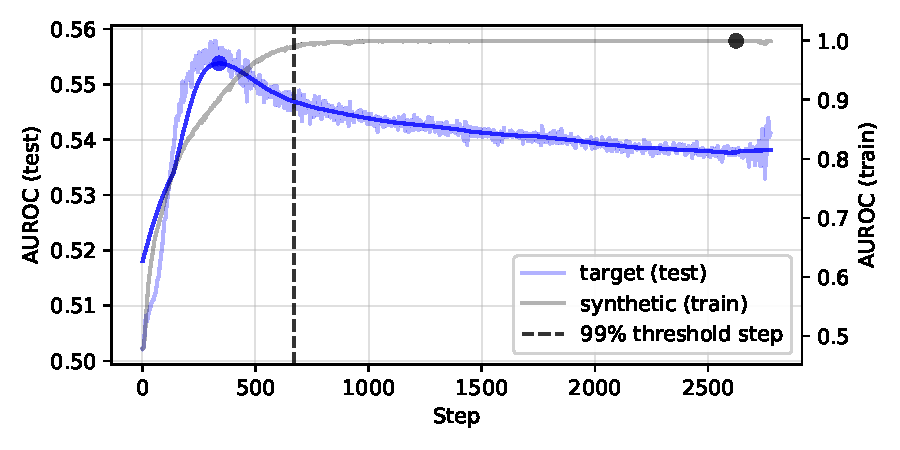
\includegraphics[width=1.0\textwidth]{figures/adsgan_uk_census_0.pdf}
  \caption{Example of ReMIA score as a function of learning step. We show the ReMIA score (AUROC) on the target records and on the synthetic data across learning steps for one of the runs of ADSGAN on UK Census dataset. The vertical dashed line represents the step when the performance on the target set is selected as the privacy score of ReMIA, which, according to the stopping criterion, is the step where the score on synthetic data reaches 99\%. In this example, the maximum value of the score on the target records (blue dot) is reached earlier than the step indicated by the stopping criterion leading to the privacy score and the maximum value on the synthetic data (black dot).
  }
  \label{remia_score_learning_step}
\end{figure}

\begin{table}
  \caption{Privacy scores (AUROC) for UK Census dataset (\%). We report mean and standard deviation over 4 different seeds.}
  \label{tab:privacy_scores_uk_census}
  \centering
  \begin{tabular}{lS[table-format=2.1(1)]S[table-format=2.1(1)]S[table-format=2.1(1)]S[table-format=2.1(1)]S[table-format=2.1(1)]}
    \toprule
    Generator & \multicolumn{1}{c}{DCR} & \multicolumn{1}{c}{DOMIAS} & \multicolumn{1}{c}{ReMIA} & \multicolumn{1}{c}{smMIA(out)} & \multicolumn{1}{c}{smMIA(med)} \\
    \midrule
    ADSGAN & \num{33.1 +- 3.9} & \underline{\num{53.4 +- 1.2}} & \underline{\num{54.1 +- 0.7}} & \multicolumn{1}{c}{-} & \multicolumn{1}{c}{-} \\
    ARF & \num{43.9 +- 1.0} & \underline{\num{57.2 +- 1.5}} & \underline{\num{62.5 +- 1.8}} & \underline{\num{80.1 +- 2.1}} & \underline{\num{64.5 +- 6.4}} \\
    Aindo & \num{46.6 +- 1.9} & \underline{\num{56.2 +- 0.7}} & \underline{\num{59.5 +- 0.4}} & \underline{\num{76.8}} & \underline{\num{61.7}} \\
    BayNet & \num{41.6 +- 3.5} & \underline{\num{53.5 +- 2.0}} & \underline{\num{52.7 +- 1.3}} & \underline{\num{80.0 +- 5.4}} & \num{58.0 +- 2.7} \\
    CTGAN & \num{11.9 +- 2.7} & \num{51.1 +- 0.9} & \num{50.9 +- 1.3} & \underline{\num{64.0 +- 1.7}} & \num{47.1 +- 2.8} \\
    PateGAN & \num{28.1 +- 1.5} & \num{52.3 +- 1.1} & \num{52.4 +- 0.2} & \multicolumn{1}{c}{-} & \multicolumn{1}{c}{-} \\
    PrivBayes($\epsilon$=10) & \num{29.0 +- 4.9} & \underline{\num{51.8 +- 1.3}} & \num{51.1 +- 1.2} & \num{56.5 +- 0.8} & \num{54.6 +- 2.9} \\
    PrivBayes($\epsilon$=1000) & \num{39.4 +- 3.2} & \underline{\num{52.7 +- 1.0}} & \underline{\num{54.2 +- 1.7}} & \underline{\num{79.3 +- 2.0}} & \num{56.0 +- 2.2} \\
    SynthPop & \num{50.2 +- 2.8} & \underline{\num{63.3 +- 1.0}} & \underline{\num{63.8 +- 1.2}} & \underline{\num{86.4 +- 2.3}} & \underline{\num{75.7 +- 2.1}} \\
    TVAE & \num{28.2 +- 8.1} & \underline{\num{53.9 +- 0.9}} & \underline{\num{56.3 +- 1.5}} & \multicolumn{1}{c}{-} & \multicolumn{1}{c}{-} \\
    TabDDPM & \num{47.4 +- 18.9} & \underline{\num{53.4 +- 2.3}} & \underline{\num{55.5 +- 1.9}} & \multicolumn{1}{c}{-} & \multicolumn{1}{c}{-} \\
    \bottomrule
\end{tabular}

\end{table}

\begin{table}
  \caption{Privacy scores (AUROC) for California dataset (\%). We report mean and standard deviation over 4 different seeds.}
  \label{tab:privacy_scores_california}
  \centering
  \begin{tabular}{lS[table-format=2.1(1)]S[table-format=2.1(1)]S[table-format=2.1(1)]S[table-format=2.1(1)]S[table-format=2.1(1)]}
    \toprule
    Generator & \multicolumn{1}{c}{DCR} & \multicolumn{1}{c}{DOMIAS} & \multicolumn{1}{c}{ReMIA} & \multicolumn{1}{c}{smMIA(out)} & \multicolumn{1}{c}{smMIA(med)} \\
    \midrule
    ADSGAN & \num{16.6 +- 4.7} & \num{51.9 +- 1.6} & \num{51.5 +- 1.6} & \multicolumn{1}{c}{-} & \multicolumn{1}{c}{-} \\
    ARF & \num{26.0 +- 6.5} & \underline{\num{52.8 +- 0.8}} & \underline{\num{54.4 +- 1.9}} & \num{53.1 +- 5.7} & \num{51.4 +- 4.0} \\
    Aindo & \num{18.9 +- 2.2} & \num{50.6 +- 0.4} & \num{51.6 +- 1.6} & \underline{\num{88.1}} & \num{50.8} \\
    BayNet & \underline{\num{74.0 +- 4.6}} & \underline{\num{73.9 +- 2.0}} & \underline{\num{80.6 +- 0.9}} & \underline{\num{81.0 +- 6.1}} & \num{53.5 +- 5.7} \\
    CTGAN & \num{9.3 +- 3.2} & \num{50.6 +- 0.7} & \num{51.0 +- 1.6} & \underline{\num{86.6 +- 4.2}} & \num{51.8 +- 3.6} \\
    PateGAN & \num{29.7 +- 16.4} & \num{50.4 +- 1.1} & \num{49.9 +- 1.1} & \multicolumn{1}{c}{-} & \multicolumn{1}{c}{-} \\
    PrivBayes($\epsilon$=10) & \num{8.1 +- 2.2} & \num{50.7 +- 0.9} & \num{51.6 +- 1.3} & \underline{\num{82.9 +- 1.9}} & \num{48.5 +- 2.5} \\
    PrivBayes($\epsilon$=1000) & \num{8.5 +- 2.4} & \num{50.7 +- 1.2} & \num{51.4 +- 0.9} & \underline{\num{84.3 +- 4.6}} & \num{48.8 +- 2.2} \\
    SynthPop & \num{41.4 +- 9.1} & \underline{\num{56.6 +- 1.3}} & \underline{\num{60.6 +- 1.1}} & \underline{\num{85.5 +- 2.4}} & \num{47.2 +- 3.1} \\
    TVAE & \num{27.9 +- 3.4} & \underline{\num{53.2 +- 1.1}} & \underline{\num{54.9 +- 1.4}} & \multicolumn{1}{c}{-} & \multicolumn{1}{c}{-} \\
    TabDDPM & \underline{\num{59.8 +- 17.2}} & \underline{\num{53.1 +- 1.5}} & \underline{\num{58.5 +- 0.7}} & \multicolumn{1}{c}{-} & \multicolumn{1}{c}{-} \\
    \bottomrule
\end{tabular}

\end{table}


\begin{table}
  \caption{Detection scores  (\%). This table reports the Detection (the lower the better) scores for all SDGs and datasets. SDGs were evaluated on a subset of 10,000 records from the original datasets, with the exception of CTGAN where we used 5,000 records. We report mean and standard deviation over 4 different seeds. See Section \ref{app:experimental_setup} for more details on how detection is computed.}
  \label{tab:detection}
  \centering
  \begin{tabular}{lS[table-format=3.2(2)]S[table-format=2.2(2)]S[table-format=2.2(2)]}
    \toprule
    Generator & \multicolumn{1}{c}{Adult} & \multicolumn{1}{c}{California} & \multicolumn{1}{c}{UK Census} \\
    \midrule
    ADSGAN & \num{99.65 +- 0.26} & \num{99.05 +- 0.26} & \num{87.12 +- 2.26} \\
    ARF & \num{97.50 +- 0.22} & \num{96.52 +- 0.10} & \num{77.35 +- 1.02} \\
    Aindo & \num{60.58 +- 1.04} & \num{68.55 +- 1.18} & \num{57.82 +- 0.40} \\
    BayNet & \num{65.92 +- 0.82} & \num{67.33 +- 0.31} & \num{80.03 +- 0.66} \\
    CTGAN & \num{99.38 +- 0.13} & \num{98.22 +- 0.17} & \num{99.67 +- 0.13} \\
    PateGAN & \num{99.80 +- 0.14} & \num{99.17 +- 0.21} & \num{90.38 +- 1.16} \\
    PrivBayes($\epsilon$=10) & \num{100.00 +- 0.00} & \num{99.25 +- 0.06} & \num{82.10 +- 2.04} \\
    PrivBayes($\epsilon$=1000) & \num{98.95 +- 0.24} & \num{97.85 +- 1.08} & \num{96.95 +- 1.14} \\
    SynthPop & \num{60.60 +- 0.36} & \num{64.30 +- 0.57} & \num{58.67 +- 1.01} \\
    TVAE & \num{99.60 +- 0.12} & \num{97.65 +- 0.17} & \num{84.55 +- 1.34} \\
    TabDDPM & \num{84.70 +- 0.42} & \num{69.30 +- 0.67} & \num{64.85 +- 0.62} \\
    \bottomrule
\end{tabular}

\end{table}

\begin{table}
  \caption{ML efficacy scores (\%). This table reports the ML Efficacy (the higher the better) scores for all SDGs and datasets. SDGs were evaluated on a subset of 10,000 records from the original datasets, with the exception of CTGAN where we used 5,000 records. We report mean and standard deviation over 4 different seeds. See Section \ref{app:experimental_setup} for more details on how ML efficacy is computed.}
  \label{tab:ml_efficacy}
  \centering
  \begin{tabular}{lS[table-format=2.2(2)]S[table-format=2.2(2)]S[table-format=2.2(2)]}
    \toprule
    Generator & \multicolumn{1}{c}{Adult} & \multicolumn{1}{c}{California} & \multicolumn{1}{c}{UK Census} \\
    \midrule
    ADSGAN & \num{-4.68 +- 1.00} & \num{-25.79 +- 3.49} & \num{-7.28 +- 0.44} \\
    ARF & \num{-2.02 +- 0.73} & \num{-15.56 +- 0.59} & \num{-4.01 +- 0.70} \\
    Aindo & \num{-1.63 +- 0.61} & \num{-10.74 +- 1.64} & \num{-0.91 +- 0.29} \\
    BayNet & \num{-0.65 +- 0.51} & \num{-2.37 +- 0.49} & \num{-7.92 +- 0.39} \\
    CTGAN & \num{-14.14 +- 2.28} & \num{-73.14 +- 1.75} & \num{-51.18 +- 3.26} \\
    PateGAN & \num{-5.99 +- 0.79} & \num{-44.45 +- 9.06} & \num{-11.48 +- 0.76} \\
    PrivBayes($\epsilon$=10) & \num{-29.68 +- 13.25} & \num{-73.93 +- 2.69} & \num{-8.87 +- 2.55} \\
    PrivBayes($\epsilon$=1000) & \num{-8.02 +- 3.26} & \num{-66.76 +- 3.57} & \num{-29.05 +- 19.54} \\
    SynthPop & \num{-1.38 +- 0.38} & \num{-9.12 +- 1.12} & \num{-1.08 +- 0.28} \\
    TVAE & \num{-3.68 +- 0.50} & \num{-17.13 +- 2.22} & \num{-5.03 +- 0.72} \\
    TabDDPM & \num{-2.52 +- 0.50} & \num{-4.96 +- 0.67} & \num{-2.22 +- 0.17} \\
    \bottomrule
\end{tabular}

\end{table}

\begin{figure}[!htbp]
  \centering
  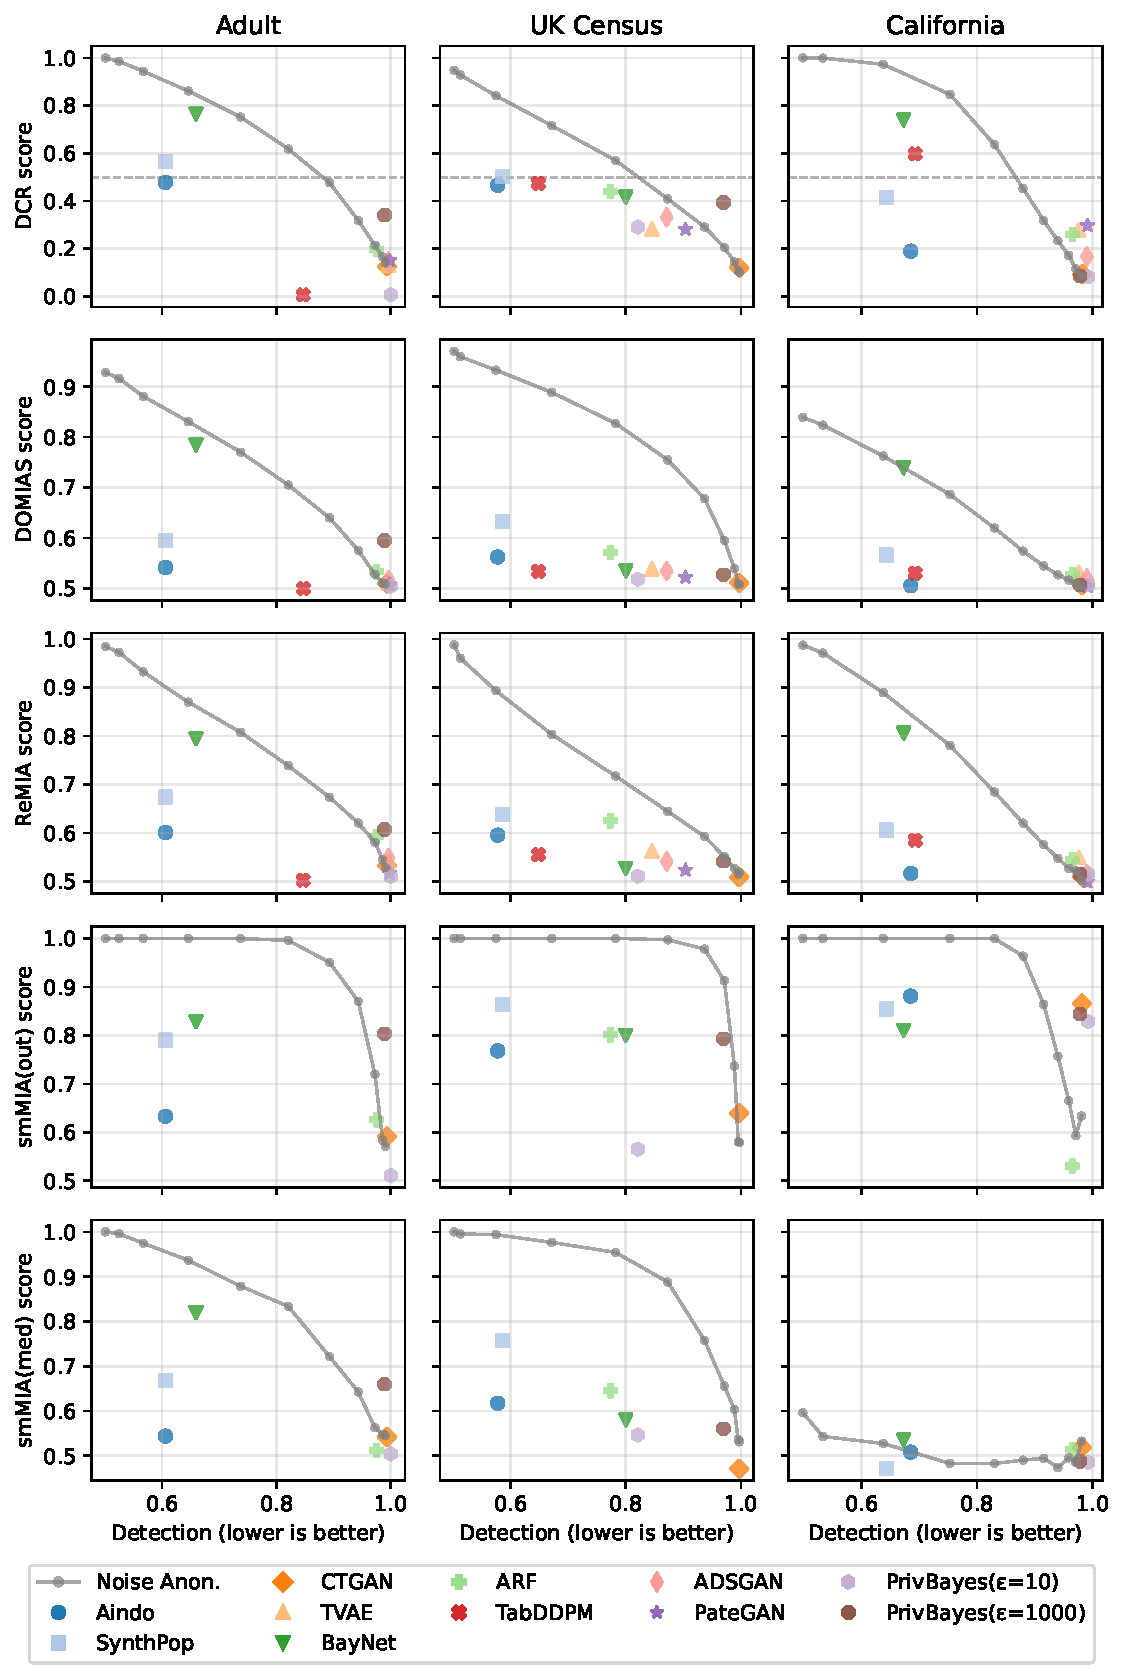
\includegraphics[width=1.0\textwidth]{figures/quality_vs_privacy/detection_vs_privacy_all.pdf}
  \caption{Privacy-fidelity trade-off. We show the fidelity of the synthetic data in terms of Detection (the lower the better) against the privacy scores (the lower the better) of the different privacy metrics for all three datasets. The gray line represents the performance of the noise-based anonymization method.
  }
  \label{fidelity_vs_privacy}
\end{figure}

\begin{figure}[!htbp]
  \centering
  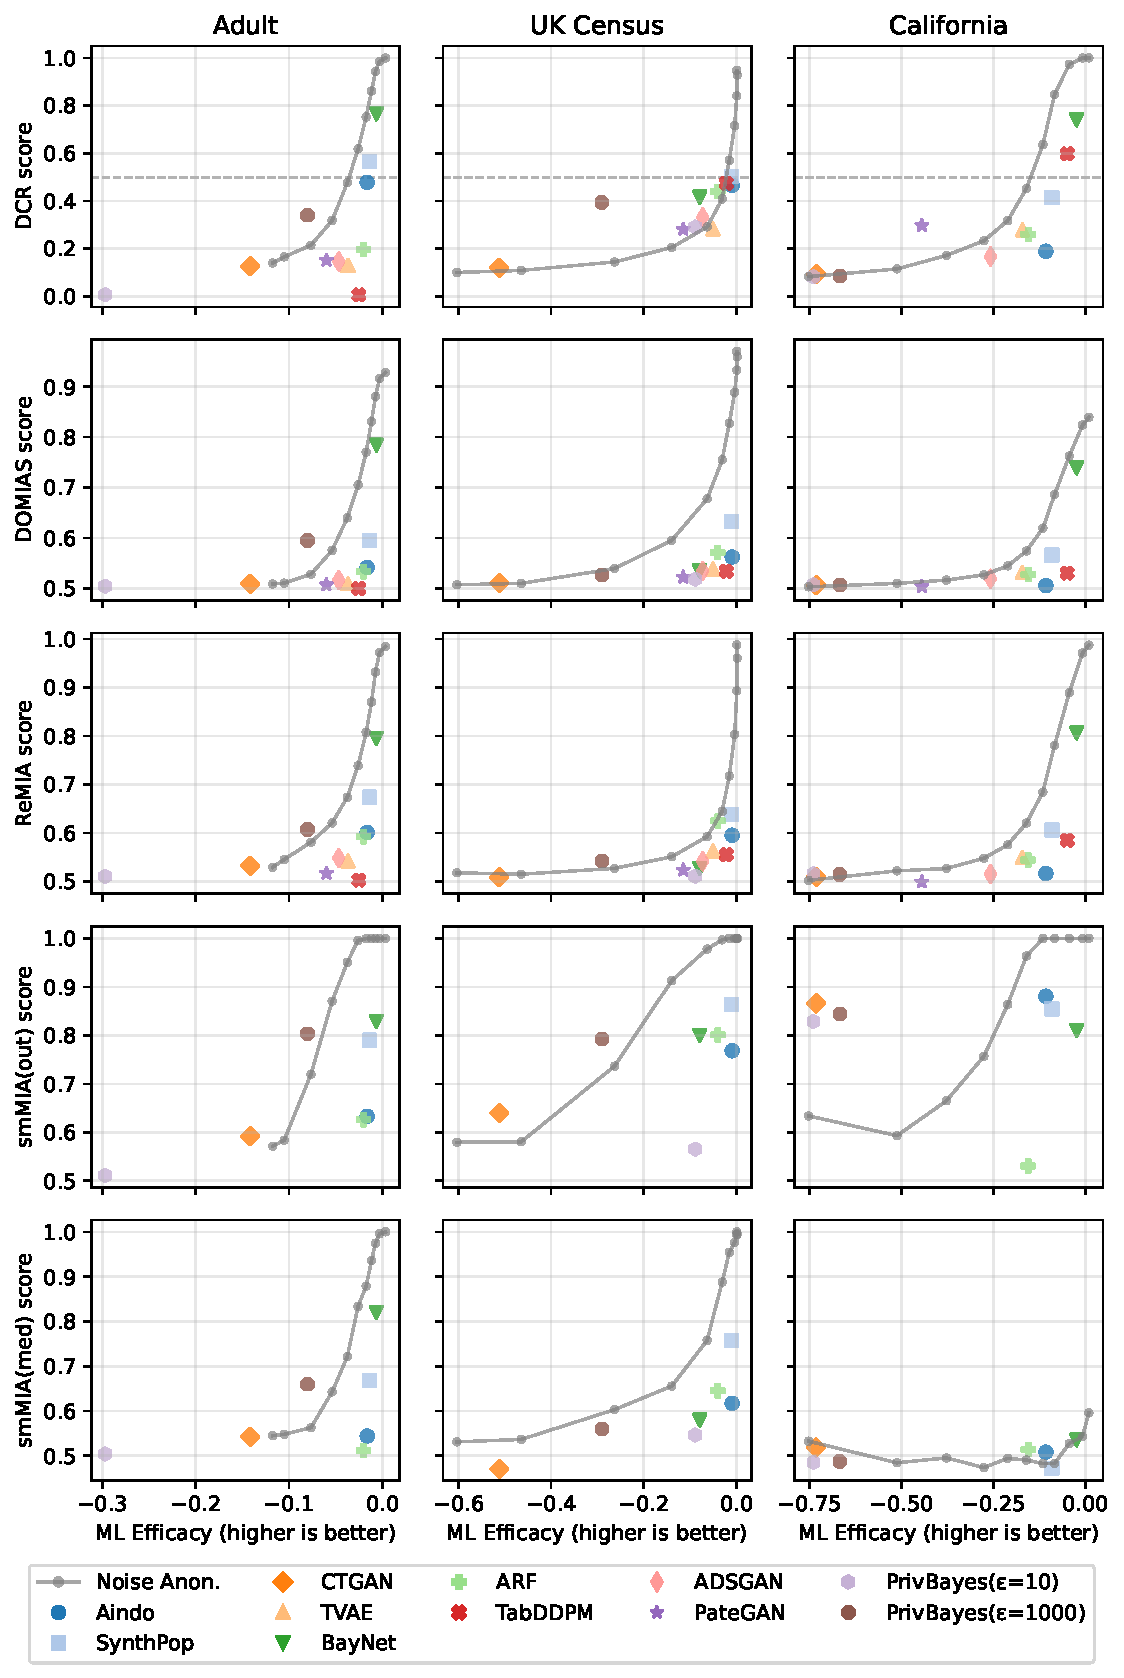
\includegraphics[width=1.0\textwidth]{figures/quality_vs_privacy/ml_efficacy_vs_privacy_all.pdf}
  \caption{Privacy-utility trade-off. We show the utility of the synthetic data in terms of ML Efficacy (the higher the better) against the privacy scores (the lower the better) of the different privacy metrics for all three datasets. The gray line represents the performance of the noise-based anonymization method.
  }
  \label{utility_vs_privacy}
\end{figure}

\begin{figure}[!htbp]
  \centering
  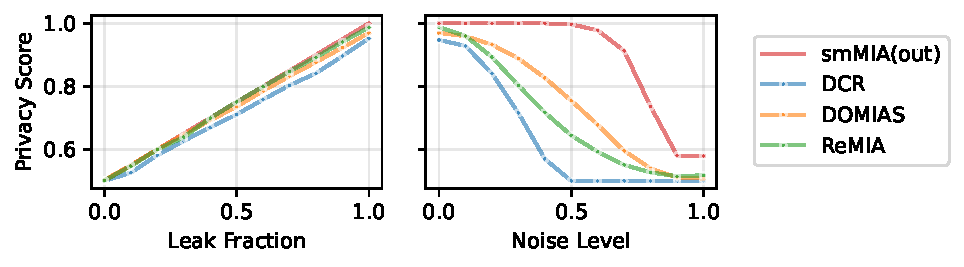
\includegraphics[width=1.0\textwidth]{figures/privacy_risk_vs_leak_fraction_and_noise_level_uk_census.pdf}
  \caption{Metrics evaluation in SDGs with controlled level of privacy risk (UK Census dataset).
  }
  \label{leak_fraction_alpha_vs_privacy_uk_census}
\end{figure}

\begin{figure}[!htbp]
  \centering
  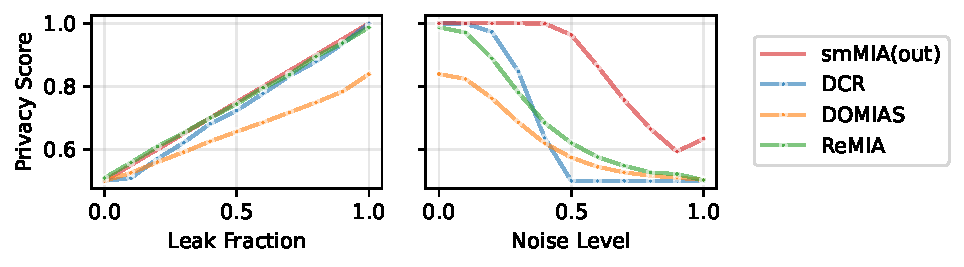
\includegraphics[width=1.0\textwidth]{figures/privacy_risk_vs_leak_fraction_and_noise_level_california.pdf}
  \caption{Metrics evaluation in SDGs with controlled level of privacy risk (California dataset).
  }
  \label{leak_fraction_alpha_vs_privacy_california}
\end{figure}


\section{Resources and Assets}

\subsection{Computational Resources}
\label{app:computational_resources}

The following hardware was used for performing the experiments in this article:
\begin{itemize}
    \item CPU: AMD Ryzen Threadripper 2950X (16-Core)
    \item Memory: 125 GiB
    \item GPU: NVIDIA RTX A5000
\end{itemize}

Running the experiments for the paper took approximately 882 hours of computational time (assuming serial execution), of which about 865 hours were spent on attacks based on shadow modeling.
We estimate that the total time taken for all experiments (including those not reported in the paper) was approximately 1500 hours.


\subsection{Assets and Code Availability}
\label{app:assets_code_availability}
Our code will be released upon publication, excluding the proprietary generative model used in our experiments.
All the assets and code used in our experiments, with the exception of the proprietary generative model, are open-source and publicly available.
We summarize the relevant assets used in our experiments and their availability in Table \ref{tab:assets_summary}.
\begin{table}[h]
  \centering
  \caption{Summary of assets used in our experiments.}
  \begin{tabular}{lcc}
    \toprule
    Asset & License & Credits \\
    \midrule
    Adult dataset & CC BY 4.0 & \citet{adult} \\
    California dataset & CC0 public domain & \citet{california} \\
    UK Census dataset & Open Government Licence (OGL) & \citet{uk_census} \\
    aindo-anonymize library & MIT License & \citet{aindo-anonymize} \\
    DOMIAS code & MIT License & \citet{van2023membership} \\
    smMIA code & MIT License & \citet{meeus2023achilles} \\
    \bottomrule
  \end{tabular}
  \label{tab:assets_summary}
\end{table}
